\documentclass[UKenglish]{ifimaster}  %% ... or USenglish or norsk or nynorsk
\usepackage[latin1]{inputenc}         %% ... or utf8 or applemac
\usepackage[T1]{fontenc,url}
\urlstyle{sf}
\usepackage{babel,textcomp,csquotes,ifimasterforside,varioref,graphicx}
\usepackage{amsthm}
\theoremstyle{definition}
\newtheorem{requirement}[equation]{Requirement}

\usepackage[backend=biber,style=numeric-comp]{biblatex}
\usepackage{datatool}
\usepackage{hyperref}
\usepackage[acronym]{glossaries}
\makeglossaries

\title{Smart phone apps for military situational awareness}        %% ... or whatever
%\subtitle{The next generation}   %% ... if any
\author{Ida Marie Fr{\o}seth}              
\bibliography{mybib}           
\begin{document}
\ififorside{}
\frontmatter{}
\maketitle{}


%\input{./content/problemDescription}
\chapter*{Abstract}                   %% ... or Sammendrag or Samandrag
The text of the abstract;
typically, 2--5 sentences.

What it is all about??
Title page, abstract, ...
%!TEX root = ../xxxx-xx-xx_idamfro_masterthesis.tex
\chapter*{Preface}                    %% ... or Forord
This thesis was written as a part of my Masters degree in Informatics at UiO. Most of the work was done in the period from August 2016 to May 2017. The thesis was done in collaboration with the FFI. 


The thesis is the original and independent work by the author, Ida Marie Fr{\o}seth and supervised by dr. Frank Trethan Johnsen and dr. Trude Hafs{\o}e Bloebaum. 


INCLUDE: How literature have been examined and where the publications have been found

%!TEX root = ../xxxx-xx-xx_idamfro_masterthesis.tex
\chapter*{Acknowlegement}
%	- Dr. Frank Tetran Johnsen 
%	- Trude Bloebaum Hansen
%	- HV(?)
%	- FIH(?)
%	- Magnus Frank
%	- review:  Gunstein Thomas Frøseth(?)
%	- Lasse Sæther

%uio and FFI
\newacronym{uio}{UiO}{the University of Oslo}
\newacronym{ffi}{FFI}{Norwegian Defence Research Establishment}
\newacronym{caged}{CAGED}{Communication Application with Geographical Element Data}

%Requirement engineering
\newacronym{re}{RE}{Requirement Engineering}
\newacronym{foss}{FOSS}{Free Open Source Software}
\newacronym{he}{HE}{Heuristic Evaluation}
\newacronym{hci}{HCI}{Human Computer Interactions}

%Military tbg
\newacronym{bft}{BFT}{Blue Force Tracking}
\newacronym{c2is}{C2IS}{Command and Control Information System}
\newacronym{hv}{HV}{Home Guard}
\newacronym{isty}{ISTY}{Rapid-reaction Intervention Forces }
\newacronym{nffi}{NFFI}{NATO Friendly Force Information}
\newacronym{fmn}{FMN}{Federated Mission Network}
\newacronym{mgrs}{MGRS}{Military grid reference system}
\newacronym{nato}{NATO}{North Atlantic Treaty Organization}
\newacronym{nbf}{NBF}{Network Centric Defence}
\newacronym{nnec}{NNEC}{NATO Network Enabled Capability}

%Technical abbre
\newacronym{byod}{BOYD}{Bring Your Own Device}
\newacronym{cots}{COTS}{Commercial off-the-shelf}
\newacronym{rest}{REST}{Representional State Transfer}
\newacronym{cde}{CD\&E}{Concept Development and Experimentation}
\newacronym{osm}{OSM}{OpenStreetMap}
\newacronym{lte}{LTE}{Long-term Evelution}


\tableofcontents{}
\listoffigures{}
\listoftables{}
\printglossary[type=\acronymtype,title=Abbreviations]

\mainmatter{}

\chapter{Introduction}
\section{Motivation}
There is no doubt that the Internet has been a great success, and the distribution of network protocols have made networks autonomous and fault tolerant\cite{SDN_Comprehencieve}. However, during the last decades, the computing trends have changed drastically \cite{ONF_SDN_Whitepaper} from being static homogeneous client-to-server communication to highly mobile and heterogeneous networks \cite{future_internet_ANA} \cite{ONF_SDN_Whitepaper}. The content have also changed from static text or web pages to include real-time multimedia and big data. In addition, the security demands are driven to a whole new level by the dependency of IT in both government, banking and transport. The change is due to the evolution of virtualized servers, the rise of cloud services, the explosion of different (mobile) computing devices and wireless communication. Since IP networks never has been developed to meet the needs of todays network, it have made them almost unmanagable and very rigid. 

///////////THIS DEFINITLY HAS TO BE REWRITTEN!/////////////////////////
The tight coupling between the control plane (the part of the network that make the forwarding decision) and the data plane (the part of the network/a switch that actually forwards a packet from one port to another) have lead to a complexity that are very expensive, static and almost unmanageable. 

In the military domain the same problem arise, and the largest problem is often the lack of flexibility and agility. 

To remove the disadvantages we have in todays network with highly coupled data / control plane and rigid configuration, the best solution is often to centralize the controller, and this is true for big data centers, but in a military context this is not always desirable  ->  because we need each node to be autonomous in case they are seperated from the core network (as they usually are). Military networks need some kind of automatic and dynamic way of assigning SDN controllers to switches. As you will see in the related work section some have tried to this before but.... maybe aiming for a different domain? 

This thesis will look at mechanisms to best solve the distribution of SDN controllers in a military context but at the same time achieve the most advantages from having the controllers centralized.

--What is wrong with todays networks and how would SDN help us?
-- What problem do we have in military networks? => New era within networking -SDN

\subsubsection{NOTES - Use cases for SDN in a military operation?}
\begin{itemize}
\item More flexible networks - save time and money
\item QoS
\item Added security (?)
\end{itemize}



\section{Derived problem description}
How to dynamically place SDN controllers in a military networks to.....?


\section{Method}
Software engineering -> lab experiment

\section{Related work}
%%%DISCO%%%
\cite{DISCO} implemeted what they called DIstributed SDN COntrol plane (DISCO) for mission-critical networks. They implemented the AMQP a message-oriented (pub/sub) middelware protocol on top of the Floodlight controller (A Messenger which subscribe to recive $Packet_IN$ from the core module / OpenFlow events, and several Agent which handles pub/sub operations with other nodes). The drawback with their solutions is that they don´t support dynamically domains. When a controller is assign a domain, they are in charge for that domain. Does not support a hierarchi of controllers. In tactical networks which are highly dynamic and XXX there is a demand for nodes being autonomous. With the solution of \cite{DISCO} it is not possible to take advantages of a centralized controller. To take advantages of centralized controll, but at the same time being autonomous it can be some sort of hierarchy similar to NTP, where stratum 0 is the top tier, and if there is a stratum 0 controller in the network, he is in charge. Else if there is only stratum 1 nodes in the network the controllers communicate and cooparate in a distributed manner. More like a ANA approach with a bootstrap method, Membership database ++(?)\cite{ana}

%%%Dynamic Resource Discovery%%%
\cite{DRDP_for_SDN} propose a method for distributing the load among controllers by developing a Dynamic Resource Discovery Protocol for Software Defined Networks as an alternative to the usual Link-Layer Discovery Protocol. 

"a protocol that allows to the controllers discover the network topology and distribute its management by themselves." 

"The process of creating the control layer is executed in two phases, the forwarding phase where the controllers announce their presence and the nodes that start the creation of the control channels (leaf nodes) are discovered, and the backward phase where the nodes decide which node to join in direction of a controller, thus creating the control layer."

"time-efficiently managed since the switches are managed by their nearest controller"

" Although this work only takes into account the delay other parameters may be considered when building the control layer."


"Recently, Google has presented their experience with B4 [1], a global SDN deployment interconnecting their datacenters. In B4, each site hosts a set of master/slave controllers that are managed by a gateway." 


%%%Bootstrapping SDN Controllers%%%
\cite{Bootstrapping_SDN_Controllers} proposed an approached called InitSDN to bootstrap the distributed SDN architecture and deploy distributed controllers. Their solution relied on dividing the network in two slices, one control slice for controlling controllers and the other for data. 

Their architecture consists of six modules (modular software). Two basic services named Discovery and Topology which is responsible for discovering of the switches and hosts by sending LLDP packets and Network Hypervisor which slice the network in control and data slice (here they used the Flowvisor - NFV controller). In addition they have four control plane configuration modules namely "control plane logic partitioning configuration", "Control Plane Logic Synchronization configuration" (uses Apache Zookeeper), "Control Plane Topology Configuration", "Host Remote Access Configuration"

"SDN architecture envisions a centralized control plane, which may result in adverse consequences to the reliability and performance [3]. Recent efforts have proposed a logically centralized but physically distributed control plane [3]."

"designed to make SDN more flexible, reliable, fault-tolerant without adding complexity to the controllers."

"InitSDN can increase or decrease the size of slices dynamically, change the topology of the controlslice, change the coordination mechanism among the controllers (e.g. use Zookeeper or Chubby, etc) to adapt to network topology changes or to dynamic network loads or simply as part of an upgrade."


%%%ElastiCon%%%
\cite{ElastiCon} 
Read more
"ElastiCon introduces a mechanism to change the active control connections from one controller to another, dynamically on run time. The mechanism defines the message exchange required to achieve the control path migration."\cite{SDN_VN_ControlPath}

"To address this problem, we propose ElastiCon, an elastic dis- tributed controller architecture in which the controller pool is dy- namically grown or shrunk according to traffic conditions. To ad- dress the load imbalance caused due to spatial and temporal varia- tions in the traffic conditions, ElastiCon automatically balances the load across controllers thus ensuring good performance at all times irrespective of the traffic dynamics. We propose a novel switch mi- gration protocol for enabling such load shifting, which conforms with the Openflow standard. We further design the algorithms for controller load balancing and elasticity. We also build a prototype of ElastiCon and evaluate it extensively to demonstrate the efficacy of our design."
Maybe we want a controller to controll another controller?

%%%SDN_VN_ControlPath%%%
\cite{SDN_VN_ControlPath} READ MORE
Network Virtualization and Virtual SDN controllers for loadbalancing. 

\section{Thesis structure}

%%!TEX root = ../xxxx-xx-xx_idamfro_masterthesis.tex
\chapter{The SMART project}
The SMART project was a \gls{cde} activity sponsored by the inspector general of the \gls{hv}, and executed by the \gls{ffi} in 2016. As stated in \cite{ep1667_bakgrunn} the purpose of the activity was to '...investigate whether commercial smart technology, primarily in the form of smart phones and/or tablets, can be used as a cheap and powerful platform for situational awareness for units that have little to no technological equipment available today.'. The goal of the SMART project was to investigate how \gls{cots} products can be used to enable information sharing with all the Armed Forces units, hence complement the current solution for information sharing. Figure \ref{fig:SMART_demo_sketch} show how the SMART solution can be connected with the current Information infrastructure and ensure information exchange with other units. The interface purposed between the server and INI in \cite{ep1667_bakgrunn} are with either using the current \gls{nffi} standard or by using service orientation as defined in \gls{fmn}. 

\begin{figure}
\label{fig:SMART_demo_sketch}
\centering
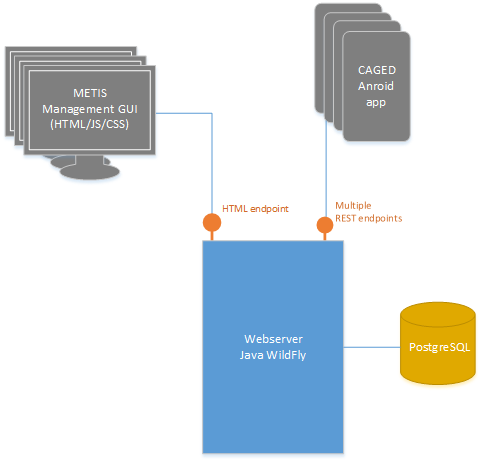
\includegraphics[width=0.8\columnwidth]{content/img/Titans_system_sketch.png}
\caption{The SMART demonstrator sketch \cite{ep1667_bakgrunn}}
\end{figure}

Through the project a demonstrator was developed and tested, and the results show that smart technology has great potential to complement the situational picture in military operations.
Through the next section the reader will get familiar with the organization and the intended user of the SMART project. Two main user groups with somewhat different requirements regarding information need, functionality and physical mobility will be identified. The second section of this chapter gives an overview of the developed prototype, its components and versions, while the last section provides an overview of the four tests that have been conducted by the SMART project. 

\section{The SMART user } \label{sec:smart_user}
The Norwegian Armed Forces are organized into five branches; the Army, the Navy, the Air Force, the \gls{hv} and the Cyber Defense. The \gls{hv} is the intended user of the SMART project and more precisely the area forces. \gls{hv} serves as a quick reaction force of the Armed Forces and their main responsibility is territorial protection. \gls{hv} consist of more than 45 000 soldiers distributed in four regions, 11 districts and 241 areas covering all over Norway\cite{forsvaret_home_guard}. The \gls{hv} is a mobilization force\footnote{Mobilization force means that the soldiers are not employed by the military on a daily basis, but train on a regular basis.} consisting of 15 \gls{isty} and 241 area forces. While the \gls{isty} are capable of rapid response and consists of highly trained and equipped personnel, the area forces have longer reaction time, are less equipped and the personnel have less training. The SMART project aims at providing a cheap communication system for the area forces, hence the user threshold has to be as small as possible, and the product has to be cheap and require as little management as possible.

\subsection{The command structure of HV}
As for any military unit, the command structure within \gls{hv} is very hierarchical see figure \ref{fig:hv_command_structure}. The smallest unit are squads which usually consists of about seven people, and are the soldiers on ground. Each squad member has a designated task and are lead by a squad leader. Squads usually operates as one unit, or at least within visual or auditory contact with their squad leader or their second in command. The squad leader executes the mission given by the platoon leader. A platoon is composed by three to five squads, which in turn are lead by the area command. Each level has one commander and one second in command. Higher up in the hierarchy there are additional roles like intelligence, operations, logistics, plans etc. 

Since the platoons are the soldiers on ground, they are highly mobile and has a rather limited information need compared to the area command staff. The area command staff, on the other hand, are usually located within a command post, are less mobile and need a broader situational picture. This leaves us with two main user groups - the \gls{hv} soldier and the staff members. The SMART project have developed two different interfaces, one for each of these user groups. The SMART Android App for situational awareness on squad and platoon level and a web interface for the staff members.


\begin{figure}
\label{fig:hv_command_structure}
\centering
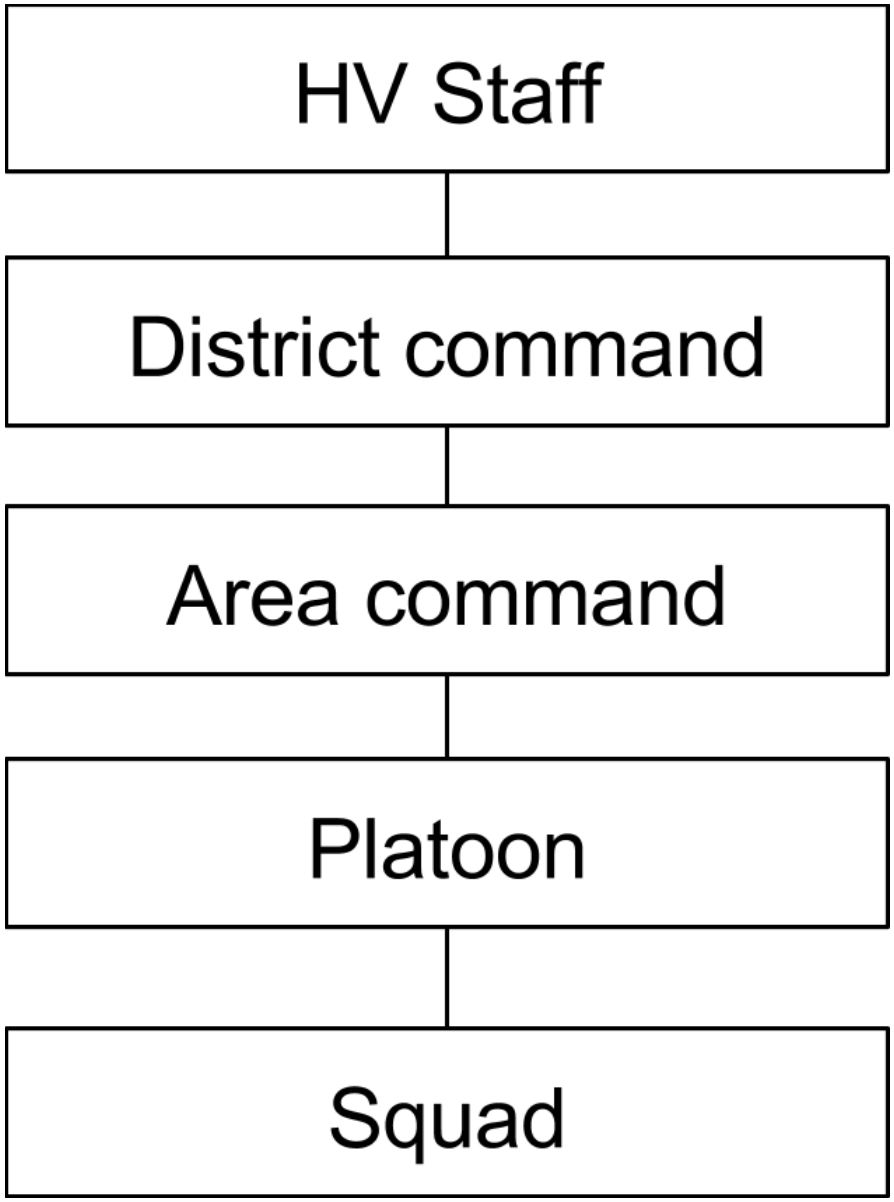
\includegraphics[width=0.4\columnwidth]{content/img/hv_command_structure.png}
\caption{\gls{hv} Command Structure}
\end{figure}

\subsubsection{The HV Soldier}
The \gls{hv} soldier is a person which have at least fulfilled one year of mandatory conscription some time in life and his/her age, background and experience can vary a lot \footnote{The age can vary from 18 - 55 years.\cite{lov_hv_2015}.} 
This accounts for both at the squad, platoon and area command level, however the commanders at each level and the people at the area command level usually have some additional training compared to the average soldier. 

\section{The TITANS and its components} \label{sec:titans_components}
The prototype developed through the SMART project is called the TITANS, and consists of three components - the smart phone App, a server component and a management interface, see figure \ref{fig:titans_architecture}.

\begin{figure}
\label{fig:titans_architecture}
\centering
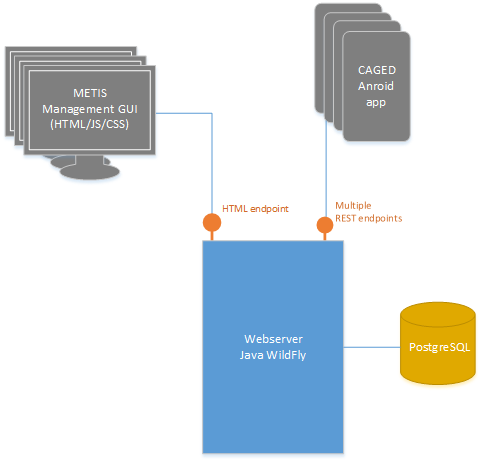
\includegraphics[width=0.8\columnwidth]{content/img/Titans_system_sketch.png}
\caption{TITANS architecture}
\end{figure}

\subsection{TITANS major versions}
Since the development of TITANS have followed an agile process the system have changed continuously. However, there are two major versions of the app to consider. The first version was developed as part of the bachelor thesis of three students from the Westerdals School of Arts, Communication and Technology during spring 2016. Their bachelor thesis \cite{gudmundsen_communication_2016} gives insight into the process of designing and developing the basic functionality for the \gls{caged} app and the server component, as well as an overview of the findings when testing it during week 17. Based on the results from this test the system was enhanced by some summer students, which implemented some major changes like adding groups, enhancing location tracking, and added the management interface called METIS. 

\subsection{TITANS security}
VPN
NFC user authentication

\section{The SMART project tests}
Table \ref{tab:smart_tests} gives an overview of the four tests that has been conducted by the SMART project. 
\begin{table}[]
\centering
\caption{The SMART project User tests}
\label{tab:smart_tests}
\begin{tabular}{|l|l|l|l|l|l|l|}
\hline
W & Location   & Duration      & Users & Ver & Activity & Comment       \\ \hline
17        & Domb{\aa}s     &  5 days              & 50  & 1  & Course & 24 h cycle \\ \hline
33        & Domb{\aa}s     &   5 days            & 42   & 2 & Course &               \\ \hline
36        & Tr{\o}ndelag  &  40 hours              & 16  & 2 & Exercise &    Used by red team\footnotemark           \\ \hline
39        & Hauerseter  & $\sim$40 hours & 33   & 2  & Exercise         &               \\ \hline
\end{tabular}
\end{table}
\footnotetext{Red team are used in exercises to train the personnel, and are playing the opponent of the blue team, the training personnel. To ensure maximum effect the red team usually gets more information (like the blue team mission and their likely movement), and the missions are usually of shorter duration.}

For all four tests, the following facts accounts:
\begin{itemize}
	\item{No user have participated on more than one test}
	\item{There have not been given any instruction on how to use the app, except a small how-to folder with the size of a credit card}
	\item{The system have been used as a tool for the soldiers to solve their main mission\footnote{This have given a valuable insight of the usability of the system.}. }
	\item{The devices have been from at least three different vendors}
	\item{\gls{ffi} have preconfigured the server and the user credentials}
\end{itemize}

From table \ref{tab:smart_tests} it is important to notice that version one was used during the first test, hence it should be given less weight when analyzing the results. It is also important to notice that the user group and the context have varied slightly form each test. During the first and second test the system was used by \gls{hv} soldiers participating at a commanders course, hence their motivation, experience and level of training can be expected to be a bit higher compared to the average user. During the third test the system was used by the red team, which differ slightly from the intended usage, however the results are still applicable. The last test is the test which is most similar to the intended usage and best represent the user group and this test should be given most weight.  

\begin{figure}
\label{fig:user_test_timeline}
\centering
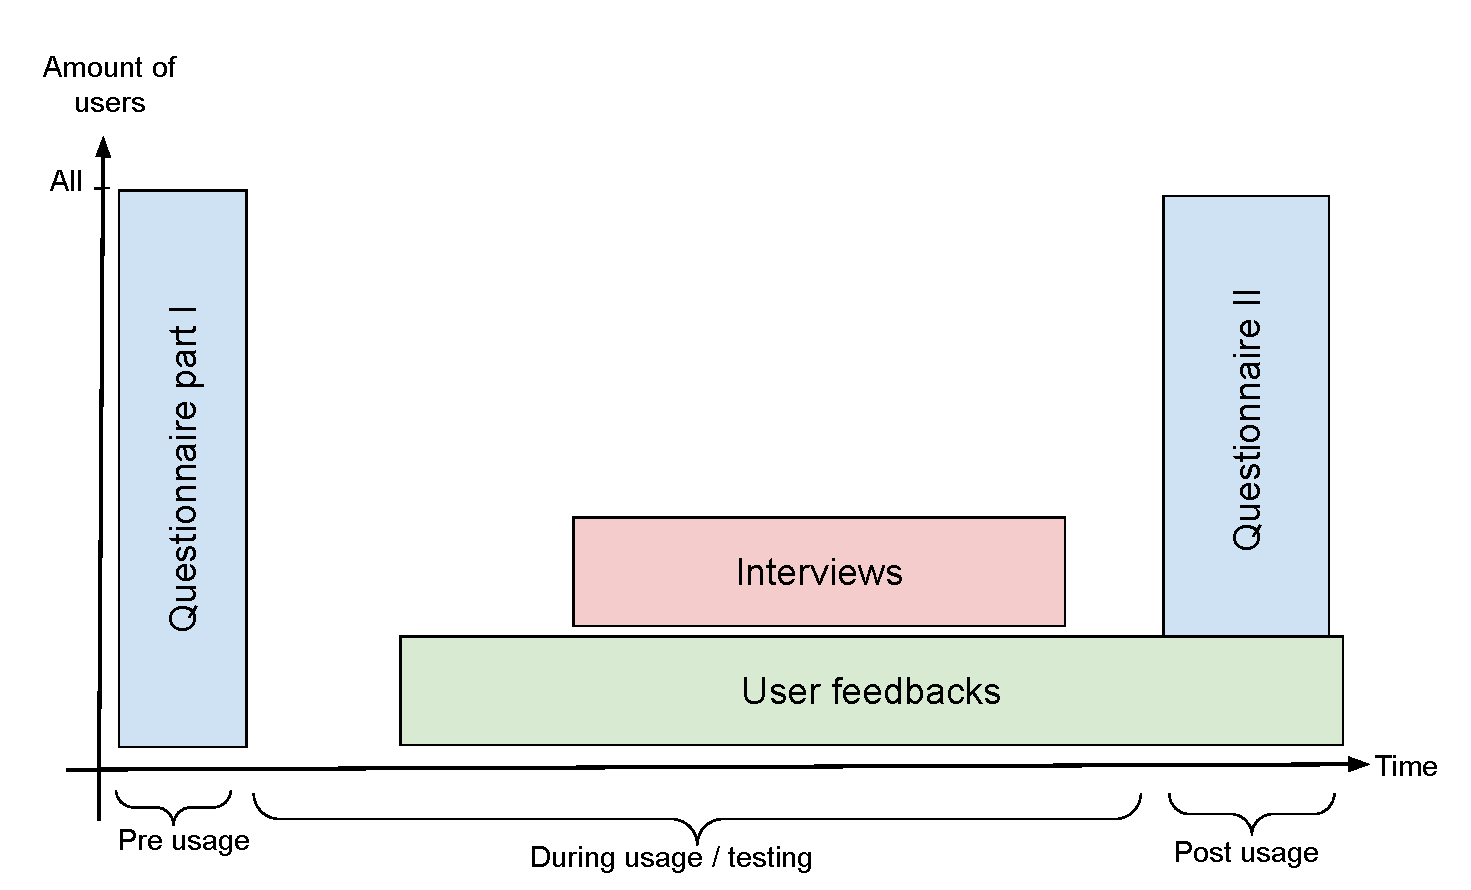
\includegraphics[width=1\columnwidth]{content/img/tests_timeline.pdf}
\caption{User test execution}
\end{figure}
Before, during and after each test a large amount of data was gathered. Figure \ref{fig:user_test_timeline} visualize the method used to gather user feedback and at what time in the test cycle it happened. As the figure shows, the methods used are questionnaires, interviews and informal conversation with the user. 



\subsection{Questionnaires}
Before and after each test, the users were asked to answer a questionnaire, referred to as questionnaire part I and part II. The questionnaires were written by some statistics experts at \gls{ffi} and included both closed-ended matrix questions and open-ended questions. The intent of the part I questionnaire was to uncover the users experience, habit and attitude of using smart technology, as well as their expectation to the developed app. The part II questionnaire gathered data about the experience from the actual usage and what potential the user saw in smart technology. 

\subsection{Interviews}
Interviews were only conducted during week 17 and 39. For the first test, a focus group of five persons were selected to represent different types of users and attitude to the system. The interviews were preformed during the execution of the test. For test two and three no formal interviews were conducted, while for the last test the user of Metis were interviewed, to gain insight into the administrator platform. 

\subsection{Other user feedback}
During the execution of the tests, a support chat room were configured enabling the users to communicate directly with the \gls{ffi}. The conversation logs both gives insight into what the user had difficulties with as well as some new requirements and proposal for enhancements were posted. In addition to the chat room \gls{ffi} met the users in different occasions both during and after the execution and in field and at the operation center. 

%!TEX root = ../xxxx-xx-xx_idamfro_masterthesis.tex
\chapter{Related work, requirement analysis and state of the art}\label{chap:analysis}
This chapter covers the requirements analysis blalblabla:-)

\section{SMART project overview}
\section{Analyzing the TITANS}\label{sec:smart_analysis}
The analyzis of the Titans form the basis for the direction and work in this thesis, and also uncover the requirements for a smart phone hosted \gls{bft} application. I have used three different approaches when analysing the system. First the data gathered by \gls{ffi} was analyzed, then a heuristic evaluation of the current solution were conductet before performing some benchmark test in order to get an overview of the system current solution. 

The rest of this chapter will first go through the findings from analyzing the user feedback, performing the heuristic evaluation and doing performance tesing. In each section a set of derived requirements and their priority will be stated. At the end of this chapter a summary of the findings is included to give the reader a overview of all the identified requirements.

\section{User experience}
The results form the questionnaires revealed that the users were very positive to both the application and the project, and all the questions regarding the idea or concept got more than 80 percent positive votes. On the question on the reason for adding information in the CAGED app, the alternative it took focus away from their main task.

The users also addresses some additional requirements to the application which can be categorized in the following categories:
\begin{itemize}
	\item{Map}
	\item{Power consumption}
	\item{Information architecture}
	\item{Location strategy}
\end{itemize}

\subsection{Map}
The users basically mentioned two main problems with the map of the current version: 
\begin{itemize}
	\item{The fidelity of the map}
	\item{The format of locations}
\end{itemize}
\subsubsection{Map fidelity}
The first issue relates to the map used in the current solution, which is \gls{osm}. \gls{osm} lacks a lot of information in some areas, and the users mentioned amongst others, contours, roads and building as examples of information which were not present. Multiple users mentioned the Norgeskart app, which uses Kartverkets open map database\footnote{http://www.kartverket.no/Kart/Gratis-kartdata/}, as an example of a good map.
The derived requirement is as follows:
\begin{requirement}
The map for such application needs fidelity similar to Norgeskart 1:50000 data set or better.
\end{requirement}

The consequences of not having an accurate map might be navigations errors, lack of trust in the system and that user rather uses other mapping applications for navigation. The consequences are crucial for the application to be used therefor this requirement should be assigned \textbf{high} priority. 

\subsubsection{Location format}
The current solution displays locations using latitude and longitude, while the soldiers are used to the \gls{mgrs}, which is also the coordinates displayed on their physical map. Since the squads still uses physical maps to navigate and the operation order usually refer to location in \gls{mgrs}, the efficiency and synergy by using the application is not as high as it could be. Since this is not a critical part of the application, but would make the soldier more efficient the following requirement should be assigned a \textbf{low} priority:
\begin{requirement}
The location of a observation or a user should be displayed using the \gls{mgrs} format. 
\end{requirement}

\subsection{Power consumption}
About one out of three users commented in the open-ended questions that their device quickly ran out of power. The devices were fully charged and each squad were given a powerbank at the start of the exercise. The duration of the tests were also relatively short compared to a real world scenario\footnote{During the first two tests the users returned their devices every 24th hour for recharging and update. While for the two last the test execution duration were only about 40 hours, see table \ref{tab:smart_tests}}. The duration of one operations usually rarely last for more than 24 hours, but the soldiers can be days without getting access to a facility with power. Often squads use vehicle for transportation, but since they were not provided with a charger for vehicles, they were not able to charge the device. The consequences of not having a device with power is crucial, and the following two requirements should have a \textbf{high} priority. 
\begin{requirement}
The smart phone app should last for at least 24 hours without the need to recharge.
\end{requirement}
\begin{requirement}
The user need to carry power resources to last for at least ***one week before returning to a facility with corded electricity. 
\end{requirement}

\subsection{Findability}


\subsection{Information architecture}
The users have through the open-ended questionnaire and in conversation pointed out multiple issues related to information architecture. There were both  

The issues can be grouped into the following categories:

Finding new information 
1 * Filtering 
2 * Feed of what is new (as of facebook being chronological)?
	- findability
3 * How to organize the information of an event




\begin{itemize}
	\item{Notifications}
	\item{Filtering information}
	\item{Visualize the situation}
\end{itemize}


\subsubsection{Notifications}
Multiple users called for a feature to be notified when there is a change in the system. Without any notification the user have to periodically check the map or the list of observations for new or updated information. This brings the soldiers focus away from their main task and are both inefficient and dangerous. If the user were notified whenever there is a change they will get a better and faster situational awareness. At the same time, if the users are constantly notified for every small change in the situation it can also draw the user attention away from their main task. In other words, the user should only be notified when the information is relevant to the user. The derived requirement is as follows:
\begin{requirement}
The user should be notified whenever relevant information\footnote{Whether information is relevant or not depends on the physical distance from the user, if the user have marked the observation as a favorite and if the user is the creator or editor of the observation with updated information.} is added or updated.
\end{requirement}

The above requirement will give an better situational awareness to the user faster, which is a core goal with the application and the requirement should have a \textbf{high} priority. 

\subsubsection{Filtering information}
Multiple users mentioned that they had problem filtering out relevant information, and this is despite the short time frame the app was used (with longer exercises more and older information would be present).  In the current solution, the idea is that an administrator (typically an user of Metis) should remove information when it gets irrelevant\cite{gudmundsen_communication_2016}. However in conversations with different users and through the interview with the Metis operator it is clear that different users with different roles have a different view of what is relevant information and not. For example would the S-2 (Intelligence) personnel of the Area Command need 'historic' information in order to analyze how the situation is evolving, while a soldier in a squad would only be interested in the information that can influence the current situation. On the other hand it is obvious that information left out (filtered) without the soldier being aware of it can be very dangerous, hence a filtering mechanism has to be user initiated and not necessary remove the information completely from the map but make it visually less important. 

Whether information is relevant or not depends on multiple factors, and using only time is not adequate; An enemy observed passing in a vehicle may only be valid for hours or minutes, while information about the location of an enemy command post would be relevant for maybe weeks, and even moths or years. The user should therefore be able to select some information to never be filtered.  

\begin{requirement}
The application should support user initiated filters which makes it visually easy to see what information is relevant. 
\end{requirement}


\subsubsection{Visualizing the situation}
This requirement is highly related to the previous requirement about filtering information, however this requirement is more related to how information is displayed. Users mentioned that they had problem seeing the view fast enough. The current solution uses clustering to avoid information overload. However the user has to zoom in to get more details about each 


Relevant information
What is the last updates



\subsection{Location preciseness}

What type of information do they have to share:
* Blue force tracking
* Observations


* In general positive to the project and the application (more than 80 percent)
* The reason for not using the app was mainly because it took focus away from their main task
*The open-ended questions and in conversation with the user, the following issues were addressed. 


\section{Heuristic evaluation}
\subsection{Why Heuristic evaluation}
\gls{he} is a informal method to evaluate the usability of a user interface design. It is conducted by simply looking at the interface and evaluate it based on some chosen design principles\cite{he_nielsen}. The advantage of the technique is that it is effective, can be used early in the development phase, is cheap and does not require to much resources \cite{Nielsen_1992_HE_method}\cite{usability_mobile_bertini}. The method also have some shortcomings as it could be biased by the current mindset of the evaluators\cite{he_nielsen}. \gls{he} should be performed independently by three to five persons as pointed out in Nielsen and Molich in \cite{he_nielsen}, however the resources available for this thesis only allowed one evaluator. 

\subsection{Choosing heuristics}
Nielsen 10 usability heuristics \cite{10_heuristics_nielsen} are well known and tested. Since touchscreen based mobile interfaces have some different \gls{hci} challenges compared to traditional computers interfaces, different set of mobile specific heuristics have been proposed\cite{kuparinen_mobile_he} \cite{usability_mobile_bertini} \cite{10_mobile_he}. \cite{kuparinen_mobile_he} propose a way to interpret the Nielsens 10 heuristics to better suit map based mobile application, and this interpretation is used when performing the \gls{he}.

\subsection{Problems discovered through heuristic evaluation}

\section{Performance testing}
\section{The domain}
* How many observation has to be supported?
* How should

The bachelor thesis \cite{gudmundsen_communication_2016} shows that when exceeding 200 observation, some devices start having problem rendering the observation. When this limit was tested, all the observation were fetched from the server every time, and since then versioning have been added, so only changed observations has to be updated.  rendering of the observations start having problems. They assumes this is sufficient, how

\section{Summary of requirements with prioritization}\label{sec:analysis_summary}


%\chapter{State of the Art}
\section{Software defined networks}
In this section I will first try to define what a \gls{sdn} are. Then we will look at different components of an \gls{sdn} like the controller, the networking element and the different \gls{api}s.
\subsection{SDN terminology and definition}
\label{sec:sdn_definition}
If you read books or papers about \gls{sdn} you would most likely find many different flavor of a definition for \gls{sdn}. Some will define it as a framework \cite{SDN_Anatomy_of_OpenFlow}, other defines it as an architecture with a centalization of the control plane \cite{SDN_Comprehensive} \cite{foundations_2015}. Nevertheless, what they usually have in common is that they define \gls{sdn} to be a way to make networks programmable by separating the control and data plane and connecting them through well defined \gls{api}s\cite{SDN_Anatomy_of_OpenFlow}. Where the dataplane is the part of the network that forward data from one port to another based on the \gls{fib} or forwarding table and the control plane is the part of the network that make forwarding decision and populate the \gls{fib}. 
\par
I will use this definition through this thesis and I would also emphasize that the location of the control plane does not have to be a single centralized controller. There are many advantages by centralizing the control plane like faster response to link failure because the information does not have to propagate through multiple nodes, loop avoidance since the controller has the complete picture, added agility when there is only one controller to configure, increased reliability due to less direct human interaction and centralized policy enforcement \cite{SDN_Anatomy_of_OpenFlow}. The obvious drawbacks are a single point of failure and attack focus, scale and latency when updating the switch which can lead to temporarily microloops (also an issue in todays networks) \cite{SDN_Anatomy_of_OpenFlow}  \cite{SDN_Comprehensive, p 48}. In addition military networks are usually connected with radio links or even sattelite with high latency and low bandwidth which amplifies the drawbacks with a centralized controller. As we will see later in this thesis there has to be some sort of dynamic controll assignment so that the network can take advantage of centralized controller when it is in a stable state but also has some kind of mechanism to function autonomously when disconnected from the controller. 
\par
Figure \ref{fig:sdn_components} shows the components of a \gls{sdn}, with the data plane which resieds on a Network element, the control plane on the \gls{sdn} controller, the management plane which are annotated as applications or services and standardised \gls{api}s to communicate between these elements. The next few section would go more in details about these component. 


\begin{figure}
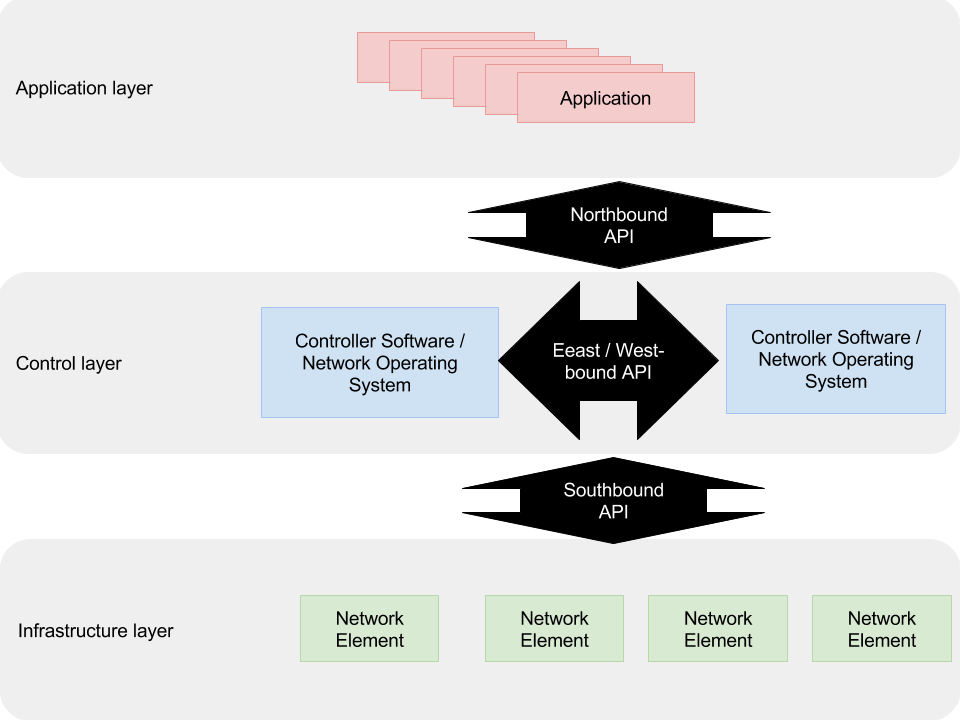
\includegraphics[width=5in]{content/img/sdn_components.png}
\caption{\gls{sdn} components}
\label{fig:sdn_components}
\end{figure} 


\subsection{Networking Element}
In traditional networks it is usual to distinguish between routers which operates on layer three and switches which operates on layer two,there are even a third class of devices known as L3 switches. The biggest difference between these devices lies in the control plane and how they get knowledge about the network and populate the \gls{fib}. When looking at the data plane all devices have the same mission - to forward data entring on one port to another port. In \gls{sdn} the control plane is logically separated from the physical data plane, hence all these devices are really just forwarding elements. 

\subsection{\gls{sdn} Controller}
======THIS SECTION HAS TO BE REWRITTEN========
The device that holds the controller logic a software defined network is often called a \gls{sdn} controller or a \gls{nos}. Many examples: OpenDaylight (open source controller) Floodlight, Cisco XNC, POX, NOX, ONOS, Beacon, Trema, Maestro, NodeFlow. There are huge differences between these controllers. Both regarding their \gls{api}s and what features they support.  


\subsection{XX-bound \gls{api}}
As mentioned in \ref{sec:sdn_definition} \gls{sdn} is about making networks programmable through well defined \gls{api}s. The purpose of an \gls{api} is to enable interaction between components, and . As figure \ref{fig:sdn_components} shows it is usual to categories the \gls{api}s in three different categories. The Southbound \gls{api} is the interface towards the networking element, and OpenFlow and Netconf are examples of open source Southbound \gls{api}s while OnePK is a Cisco propiritary protocol. The Northbound \gls{api} is the interface of the controller towards applications or services. These \gls{api} make some abstractions so the application should not have to care about the detailed configuration of the networking element. A often used Northbound \gls{api} are \gls{rest} \gls{api}. A \gls{rest} \gls{api} often communicates over HTTP and uses a standard representation format like \gls{json}, \gls{html} or \gls{xml}. Other Northbound \gls{api}s are programming languages like JAVA or propritary \gls{api}s. The East / Westbound \gls{api} are \gls{api}s to communicate between \gls{nos} or Controllers SDNi, BGP, AMQP.


\subsubsection{OpenFlow}
OF protocol, instruction set, architectue => interface\cite{sdn_Anatomy_of_OpenFlow} 

OF components:

\subsection{ONOS controller} 

\section{Distribution}
\subsection{Techniques}
\subsection{Leader Election}
\subsection{Synchronization}

\section{Federated Networks}
\subsection{Federated Mission Network}
\cite{http://www.act.nato.int/fmn}
\gls{fmn} and \gls{jmei}. Define number plans and protocols for how to connect to each nation. BGP, NTP, SNMP, ... Five service: Each nation has to manually configure their BGP peers before each . 

Four leel of capability, Mission Network Element (MNE), Mission Network eXtension (MNX) - self served but may not include sufficient mission essential services, Hosted User, other entities


FMN Affiliate : " NATO and Non-NATO nations are encouraged to become FMN Affiliates, which implies they will maintain and further develop capabilities for federated mission networks and ensure CIS security and interoperability compliance with FMN standards and principles. FMN Affiliates will be able to contribute FMN-ready forces to a mission on short notice and with minimal preparation."

\subsection{Protected Core Networks}
\section{TACOMS}
\section{TACOMS}
\gls{tacoms} was a multinational initiative with the goal to specify how \gls{nato} nations should connect in order to achieve interoperability in military operations on a tactical level. 
The next section will briefly take you through \gls{tacoms} more than 30 years of history, including the different versions of the framework called \gls{tacoms} phase 1, \gls{tacoms} phase 2 and \gls{tacoms}+. In the following sections the overall architecture of \gls{tacoms}+ will be explain together with a detailed description of the autoconfiguration specification for \gls{tacoms}+. The technical details for the other \gls{tacoms} specifications are not relevant in this thesis. I will conclude this section with my own thoughts regarding the design of \gls{tacoms} autoconfiguration specification including the advantages and weaknesses. 
\subsection{History}
\gls{tacoms} was established in 1985 as a multinational initiative by 12 \gls{nato} nations \footnote{Belgium, Canada, France, Germany, Italy, The Netherlands, Norway, Portugal, Spain, Turkey, United Kingdom and United States}. The nations saw the requirement for a new NATO standard for telecommunication due to the rising need for interoperability in the battlefield. \footnote{\gls{tacoms} were not restricted to NATO nations, but included Partnership for Peace nations. Sweden and Finland joined in 2007 when signing the 2nd \gls{mou}.} \footnote{Poland was part of \gls{tacoms} for a short period of time from 2003 to 2007 when the 2nd amendment of the \gls{mou} was signed.} \cite{https://www.tacoms.org/pages/history.aspx}. In June 2010 \gls{tacoms} phase 1  \gls{stanag}s (STANAG 4637 - 4647) were successfully promulgated as official \gls{nato} standards \cite{https://www.tacoms.org/pages/about.aspx}.The STANAG 4637-family define a protocol suite and addressing scheme for the physical layer up to the transport layer in the \gls{osi} model in addition it describe how \gls{voip} should be handled up to the application layer. However only the Netherlands implemented the STANAG 4637-family \gls{tacoms} in their tactical communication system. I think one reason for this was that some of the protocols were at the end-of-life when the STANAGs were finally finalized, like the H.323 signalling protocol which lost terrain against \gls{sip}. Another reason can be that \gls{nato} started their own standardization project for information sharing and interoperability namely the \gls{fmn}, which was based on the success and lessons learned from \gls{amn} \footnote{the operational NATO network in Afghanistan} \ref{sec:fmn}. . 

After completion of  the STANAGs in 2010, \gls{tacoms} continued as \gls{tacoms} phase 2 with a \gls{mou} / agreement ending in 2012. With phase 2, the first flavor of \gls{sdn} or programmable networking were introduced with the \gls{sow} 6 - Flexibility, Agility and Scalability \ref{sec:sow6}. Some nations withdraw from the project when entering phase 2, due to \gls{fmn} and other reasons (lost thrust because of the time it took for STANAG 4637 to come to life).  By end of the second \gls{mou}, \gls{tacoms} decided to change the strategy from writing STANAGs to rather contribute to the \gls{fmn} work. The same year \gls{tacoms} phase 1, with some quick wins (like replacing H.323 with SIP), was accepted as the transport layer for \gls{fmn}. The third \gls{mou} was signed and later extended until March 2016 in order to complete the work \footnote{Norway, Spain, Turkey, UK, Sweden, Finland, The Netherlands signed the extension. Italy withdraw, but participated in some of the work}. 

( 
Proof of concept at the \gls{cwix} exercise in 2015 in Bydgoszcz, Poland.
SDN track within FMN?
 
)

\gls{tacoms} work group finalized their work during March 2016. 

Lost many nations when they needed an extended MOU (Italy, Germany while Canada, USA exit earlier) 
 continued 2014-2016 

\subsection{TACOMS+ Technical}
\subsubsection{Architecture}
 %%%%%%EVERYTHING IS COPIED FROM TACOMS ARCHI%%%%%%
“While implementation of the UNI was national concern, implementation of NIP is coalition concern. Therefore, functions and protocols exchanged across the NIP are standardized in a detail.” 
“What does TACOMS+ provide?
TACOMS+ provides the standards that enable seamless interoperability at network domain between differing national networks to effectively create a single, coherent Mission Network. TACOMS+ creates the interface between national networks but does not impact on the national systems or capabilities. TACOMS+ utilises open standards and industry best practice to define the interoperability interfaces and the TACOMS+ standards provide the recommendations and approaches to be taken when implementing those protocols. TACOMS+ is therefore not a bespoke hardware solution, neither is it a system or a stand-alone item of equipment.”
\cite{tacoms_architecture_concept}

The different areas in TACOMS are covered by a number of profiles. Each profile is documented in one or more documents. The documents have been produced by sub teams of TACOMS, called Statement of Work (SoW), as an answer to the statement of need (SoN) decided by TACOMS PSG for each team.

Area
Profile
Documents
Technical specifications, implementation examples etc
Network Infrastructure/ Network services
Dual Stack
CL Forwarding Routing
Autoconnectivity
CL Forwarding Auto Connectivity
Bearers Transmission Mediation
(moved from CL Forwarding)
CO communication
CO Forwarding
Future bearers
Bearers -----
Voice


CO Forwarding
FMN Spiral 1 for Media
Addressing
Addressing
CL Forwarding -  Address and Numbering Plan
Network Support Services
Name Resolution
Network support services- Name Resolution
Time Synchronization
Network support services- Time Synchronization
Security
Border Protection System 
CL Forwarding Border Protection System
Public Key Infrastructure
Network support services- Public Key Infrastructure
Authentication
CL Forwarding Authentication

\gls{tacoms} includes two different automatic -> “autoconnectivity” and “service announcement”. Autoconnectivity includes discovery peers, mutual authentication and automatic peering of GRE tunnels, BGP routing and multicast routing. 

\subsubsection{Autoconnectivity}
\gls{tacoms} autoconnecitivity technical specification \cite{tacoms_t6_autoconf_techspec}
BGP, GRE, MSDP,
The entities are successfully authenticated with IKE over IPSEC. 
\gls{tacoms} autoconnectivity technical specification \cite{tacoms_t6_autoconf_techspec} divides the process for autoconfiguration in three phases: discovery, authentication and automated configuration of peers. Phase one and three rely on routing-protocols to share configuration information and a custom software to use this information to configure peers, while phase three rely on IKE over IPsec.


\subsubsubsection{Discovery}
PRECONFIGURATION:
The nodes are preconfigured with a 111.[Entity_number].x.y/8 IPv4. 
Used as source for RIPv2 packets and later as source / destination for the GRE tunnel between the nations. 
RIPv2 with
Pre-shared key and MD5 authentication
Announced 110.[Entity_number].x.y/32 address 
This network is not used for anything, only to announce the physical destination address of the GRE-tunnel (111./8 address). 

=> The Discovery phase is used to discover other \gls{tacoms} nation by announcing a /32 subnet with RIPv2. With the second octet identifying the entity it is possible to decide who would serve as a master and slave in the preceding steps. MD5 authentication with pre-shared key are used to reduce DoS attacks. 

With the extracted source of the RIPv2 announcement it is possible to start configuring a GRE tunnel with IPSEC adding the physical source and destination. The nation with the highest entity number serves as the master and start to configure the logical address of the tunnel. IPv6 is enabled at the tunnel endpoint which will enable RIPng packets to start flowing, hence phase two and autoconfiguration. 
 

The interface meant for \gls{tacoms} connectivity are configured with a  address where the second and this octet identify the nation.



The spec claims that - “This document uses the address plan designed by the SoW6-group. The discovery mechanism is not bound to that exact address plan, and can be adjusted to cohere with other address plans. When IPv6 becomes the dominant network layer technology, the entire address plan and the auto-discovery mechanisms should be updated to utilize new functionality in IPv6. “  however to identify a configuration announcement / service announcement feature it rely on the  on the script / nation software  



 \cite{tacoms_t6_autoconf_techspec}

\subsubsubsection{TACOMS Design choices}
\cite{T6-Concept_options} “...rationale for the design choices of TACOMS SON 6 group” = > Autconfiguration.
Authentication:
Options
X509v3 certificates 
Phase 1 Discovery Protocol:
Options
Custom protocol and mDNS = not part of COTS feature set. 
OSPF
RIPv2 
IPv6 Routing Protocols
Phase 2 Service Announcement Protocol
Options
Custom protocol
IPv4 Routing protocols
OSPF for IPv6
RIPng
Service Announcement
Options
DNS
UDDI
BGP



%%%%%%%%%%%%%%%Netconf survey START%%%%%%%%%%%%%%%%%
\cite{http://blog.ipspace.net/2015/10/survey-vendor-netconf-and-rest-api.html}
Routers
Vendor
NETCONF
Pure XML?
REST API
Alcatel Lucent
Yes


?
Brocade MLX
Yes


?
Cisco IOS / IOS XE
Yes
Some
No
Cisco CSR 1000V
Yes
Some
Yes (JSON)
Cisco IOS XR
Yes


?
Juniper
Yes
Yes
Yes
Updates:
IOS XR has NETCONF;
REST API is only available on CSR 1000V, not on IOS or IOS XE in general;
Juniper MX routers have REST API in Junos release 15.1;
Brocade MLX routers and ALU routers have NETCONF support;

%%%%%%%%%%%%%%%NETCONF Survey END%%%%%%%%%%%%%%%%%


---DRAW PROTOCOL in VSD----

RIPv2 - discovery (with pre-shared key)
RIPng - autconf (Over GRE tunnel 
GRE w/Ipsec - Authentication

\subsection{TACOMS+ Thoughts}
\subsubsection{Advantages}
Rely on existing standards
Except the software / script that are triggered by an autoconf event, all the code is configuration of existing standards
Introduces agility and flexibilty to FMN in a secure (?) manner
Tested 
Though at every exercise something failed

\subsubsection{Critique}
\gls{tacoms} autoconfiguration has a very “dirty” design, this is due to the inflexibility to future changes, mixing of concerns, highly coupled and dependent, duplication of functionality and lack of abstractions. 

%INFLEXIBLE%
\gls{tacoms} encapsulate information in IPv6 addresses to share configuration information,. An IPv6 address is 128 bits long, where the first 32 bits are used to identify the type of information being encapsulated. This leaves 96 bits for configuration information, and in most cases they use additional 16 or 32 bits to identify the entity sending the information. Even though \gls{tacoms} has proved that this information serves the purpose for configuring both \gls{gre}, \gls{msdp} and \gls{bgp}, it makes the protocol inflexible to future changes. What if \gls{fmn} decides to change the routing protocol? What if the length of the telephone number i changed, exceeding the length of an IPv6 address? With the method of encapsulation information in IPv6 addresses \gls{tacoms} makes the protocol inflexible to future changes in other part of the framework. (makes it also dependent upon IPv4 - how do you encapsulate a IPv6 within IPv6???). 
To make things happen faster they have to tweak the timers of the \gls{rip}, \gls{ripng} and \gls{bgp}.  = > Now 60 sec for peering. 
Dependent upon the addressing scheme

%MIXING OF CONCERNS%
\gls{bgp} is both used for announcing regular IPv6 routing information and \gls{tacoms} configuration information. The Service announcement routes are fake and not routable. \gls{tacoms} specify these routing processes to be separated, but this will actually in many cases mean an additional bgp router or software router (Cisco, as example, only support one bgp routing instance in each \gls{vrf}, and one tunnel can only have one \gls{vrf}...) %%%CHECK REF%%%%

%Dependencies%
\gls{tacoms} rely on \gls{rip} for discovery, \gls{ripng} for sharing peering information and \gls{bgp} for service announcement. Even though these protocol have been around for a while and would most likely not change in the future, it is not a good design principles to rely on these protocols.
Tacoms software would
Much static / pre-configuration that needs tweaking / workarounds of a regular router to work
Since there are so many protocols involved in the autoconfiguration process there is a need for a lot of preconfiguration/static of the IOP.
Some of the pre-configuration needs workarounds (eks when having more than one interface means having the same ip subnet for multiple interfaces on a router) because it is not standards procedure.
Injecting non-existing network addresses by adding loopback addresses. 

%Lack of abstractions and high coupling to the underlying HW%
Lack of abstraction => Not possible for a collaborative software development, and reuse of software. 
The implementation is highly dependent on the underlying HW / SW implementation. 

Many protocols used for other purposes than its original design
TACOMS uses RIPv2 for discovery, but it is not the announced address which is of interest but the source of the routing information. 
RIPng to share GRE tunnel address, Multicast information
link-by-link (not redistributed
BGP IPv6 for service annoucement (encoded by FD00:<serviceId>:<NationId>:<NationDomain>:)
TACOMS also specify regular IP v4/v6 forwarding with BGP and demands that the nation uses two different routing instances, one for forwarding and one for SA.
Not consistent - in some situation you only uses the announced ip address and other also the announced next-hop address.
Some are redistributed depending on the service ID.
=> Has to “inject” ipv4/ipv6 addresses that are not addressable
Latency of convergence because of timeout and trigger interval of the different protocols
Rely on pre-shared certificates
Maybe not possible to avoid if you will keep it secure
Error prone conversion of IPv6 addresses 
Both hex-bin, hex-decimal in the same operation
Depending of the prefix length and the announced service, what part of the address which are hex-bin and hex-dec are changes. 
Depends on the prefix mask and how the ipv6 address is represented (if aggregated with :: for 0000 for example)
Inconsistency of address allocation
Master node is the node with the largest entity number, and is the one deciding the interface addresses. 

BGP to share information. SOW6-8. Delivered the first STANAG TACOMS phase 1 in 2010. TACOMS+ next phase. Terminated March 2016. IPO opened in 1998 \cite{tacoms.org}.  8 Statement of Needs. Architecture, Phase 1 QuickWins, Reference implementation, Support to NATO FMN, Security, Agility and Flexibility, CO Services, Future IOP Bearers and Interfaces. Based on standard routing protocol to share information. RIP, RIPng and BGPv6. 


%!TEX root = ../xxxx-xx-xx_idamfro_masterthesis.tex
\chapter{Design of an enhanced solution}
\label{chap:design}
\section{Overview}
\section{Improving performance}
\section{Improving usability}
\subsection{Map}
\subsection{More precise location}


%%!TEX root = ../xxxx-xx-xx_idamfro_masterthesis.tex
\chapter{Test setup}
\label{chap:test}
\section{Heuristic evaluation}
\section{User tests}
\section{Lab tests}
%!TEX root = ../xxxx-xx-xx_idamfro_masterthesis.tex
\chapter{Evaluating the results}
\label{chap:evaluation}
\section{Evaluating the user experience}
\section{Evaluation the performance}
%!TEX root = ../xxxx-xx-xx_idamfro_masterthesis.tex
\chapter{Conclusion}\label{chap:conclusion}
\section{Future work}

\printbibliography
\input{content/Appendix}

\backmatter{}


\end{document}
